In diesem Kapitel werden für die Regression spezifisch die Erkenntnisse behandelt und erläutert. Dazu werden zuerst das Deep Cascade und 
das Direct Cascade Netzwerk vorgestellt, um dann Vergleiche zwischen der Cascade TF, Cascade und der Komplettversionen der Netze bezüglich 
vielen und wenigen Targetdaten herzustellen. Dabei wird festgestellt, dass es klare Unterschiede zwischen Deep und Direct Cascade gibt, es aber 
insgesamt funktioniert. Hier werden abschließend die Early-Stopping Metriken angewandt und dessen Ergebnisse erläutert. \\

Hier werden die beiden Regressionsnetze vorgestellt. Beide haben als Input Tabellen mit drei Spalten. 
Welche das genau sind, wurde oben bereits erklärt. Sie haben ebenfalls beide den Adam Optimizer mit der Mean Squared Error-Lossfunction. 
Als Outputlayer wird für Regression typisch ein einzelnes Linear Layer mit einer Node und der Linear Activation Function genutzt. 

\begin{figure}[htpb]
    \centering
    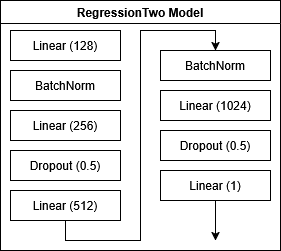
\includegraphics[height=6cm]{../../Graphiken/regressiontwo_2.png}
    \caption{\label{fig:regr2} 
    \small{Hier ist das Regr2-Netzwerk im Detail zu sehen. Die Layerreihenfolge ist von oben nach unten und folgt dann dem Pfeil. Hinter Linear 
    steht die Anzahl an Nodes und hinter Dropout wieviele prozentual beim Training nicht betrachtet werden.}}
\end{figure}

In Figure \ref{fig:regr2} ist das Regr2-Netzwerk mit allen seinen Layern. Dies ist ein Deep Cascade Netzwerk. Es wird also Layer für Layer trainiert. 
Dabei ist die Zahl hinter Linear die Anzahl der Nodes und die Zahl hinter 
Dropout die Prozente bezüglich dem Wert eins, die während des Trainings pro Epoche wegfallen. 

Das 1Lay-Netzwerk ist das Direct Cascade Regressionsnetz. Dieses hat nur ein Hiddenlayer mit einem Linearlayer mit 128 Nodes. Die 
Aktivierungsfunktion in diesem Layer ist Relu. Es wird iterativ genutzt und zwischen den Netzen Wissen mittels eines Augmented Vectors als 
neuen Input übertragen. 
Dieser wird mit der Prediction des vorherigen Netzes berechnet, indem diese als neue Spalte in der Inputtabelle des bisherigen Inputs hinzugefügt 
wird. Dies ist der Augmented Vector, der als neuer Input für das nächste Netz dient. 
